\documentclass[border=10pt]{standalone}
\usepackage{tikz}\usepackage{amsmath}\usetikzlibrary{arrows.meta}
\begin{document}
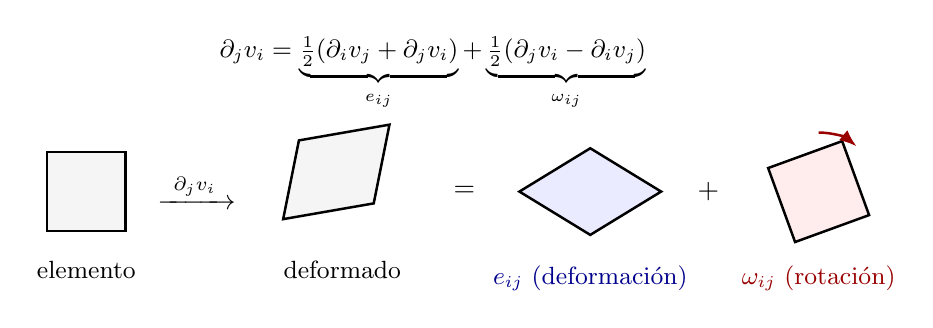
\begin{tikzpicture}[line width=0.9pt,>={Latex[length=2.2mm]}]
  % original
  \draw[fill=black!4] (0,0) rectangle (1,1);
  \node at (0.5,-0.5){\small elemento};
  \node at (1.9,0.5){$\xrightarrow{\ \partial_j v_i\ }$};
  % general: paralelogramo rotado y cizallado
  \draw[fill=black!4] (3,0.15) -- (4.15,0.35) -- (4.35,1.35) -- (3.2,1.15) -- cycle;
  \node at (3.75,-0.5){\small deformado};
  \node at (5.3,0.5){$=$};
  % deformacion pura (simetrico): diamante simetrico
  \draw[fill=blue!8] (6.0,0.5) -- (6.9,-0.05) -- (7.8,0.5) -- (6.9,1.05) -- cycle;
  \node[blue!55!black] at (6.9,-0.6){\small $e_{ij}$ (deformación)};
  \node at (8.4,0.5){$+$};
  % rotacion pura (antisimetrico): cuadrado rotado
  \draw[fill=red!7,rotate around={20:(9.8,0.5)}] (9.3,0) rectangle (10.3,1);
  \draw[->,red!60!black] (9.8,1.25) arc (90:50:0.75);
  \node[red!60!black] at (9.8,-0.6){\small $\omega_{ij}$ (rotación)};
  \node at (4.9,2.0){\small $\partial_j v_i=\underbrace{\tfrac12(\partial_i v_j+\partial_j v_i)}_{e_{ij}}+\underbrace{\tfrac12(\partial_j v_i-\partial_i v_j)}_{\omega_{ij}}$};
\end{tikzpicture}
\end{document}
